\documentclass[letterpaper,12pt]{report}
\usepackage{thesis}

\usepackage{amsmath}
\usepackage{amsmath}
\usepackage{amsfonts}
\usepackage{amssymb}

\usepackage{hyperref}

%\textwidth 5in

\newcommand{\shorttitle}{State of Practice for Medical Imaging Software}
\newcommand{\fulltitle}{Assessing the Current State of the Practice for Medical Imaging Domain within Scientific Computing Software}
\newcommand{\authorname}{Ao Dong}

\begin{document}

\pagenumbering{roman}

\thesisshorttitle {\MakeUppercase{\shorttitle}}

\thesistitle
	{\MakeUppercase{\fulltitle}}
	{\MakeUppercase{\authorname}.}
	{Master of Engineering in Computing and Software}
	{\copyright \ Copyright by Ao Dong, August 2021}

\descriptivenote{a descriptive note}

\addcontentsline{toc}{chapter}{Abstract}
\begin{center}
\textbf{\large Abstract}
\end{center}

We present a method to assess the state of the practice for software in Scientific Computing (SC) domains and apply the method to the Medical Imaging (MI) domain. This method guided us to select 29 MI software projects from 48 candidates, assess nine software qualities by answering 103 questions for each software, and interview eight of the 29 development teams. The results helped us with revealing the current status of MI software development, such as the merits, drawbacks, and pain points during the development process and the software qualities. Based on our findings, we suggested guidelines and recommendations for future SC software development. \newline

\noindent\textbf{Keywords:} Medical Imaging, Scientific Computing, software engineering, software quality, Analytic Hierarchy Process, developer interview
\addcontentsline{toc}{chapter}{Acknowledgments}
\begin{center}
\textbf{\textup{\Large Acknowledgments}}
\end{center}

acknowledgements here
\include{03contents}

\pagestyle{fancy}
%\fancyhf{}
\renewcommand{\headrulewidth}{0in}
\chead{MEng Thesis - \authorname - McMaster - Computing and Software}\ \   
\lhead{}
\rhead{}

% \pagestyle{headings}
\markboth{MASc Thesis - \authorname - McMaster - Computing and Software}{}

\pagenumbering{arabic}

\chapter{Introduction}
\label{ch_intro}
We define Scientific Computing (SC) as ``the use of computer tools to analyze or simulate mathematical models of real world systems of engineering or scientific importance so that we can better understand and predict the system’s behaviour" \cite{Smith2006}. Many researchers consider SC as the third pillar of science and engineering, along with theory and experiment \cite{Landau2005}. Almost all areas in science and engineering use computers for modeling \cite{Golub2014}, and software plays an essential role in modern scientific research \cite{Hannay2009} \cite{Wilson2014}.  Software development in SC depends on three fields of knowledge: engineering or scientific domain knowledge, mathematical algorithm knowledge, and computational algorithm knowledge \cite{Landau2005} \cite{Mehta2015}. Thus, most SC software developers are scientists in SC domains \cite{Wilson2014}. However, they do not always use the modern software development techniques, tools, and methods \cite{Wilson2014}. Therefore, we developed a methodology for assessing the state of the practice for SC software. We apply this process to Medical Imaging (MI) software that belongs to a specific domain of SC.

This report analyzes the state of the practice for MI software. MI is the clinical tool to image the interior of a body, providing information for diagnostic, analytic, and medical applications \cite{FDA2021} \cite{enwiki:1034887445}. MI is an essential part of collecting accurate information during clinical diagnosis \cite{Zhang2008}. MI software aims to visualize and process medical images and produce clinically meaningful information \cite{enwiki:1034877594}.

We aim to study the current status of SC software development in the MI domain; understand the current merits, drawbacks, and pain points during the development process, as well as the software qualities in the domain; provide guidelines and recommendations for future development.

Section \ref{sec_motivation} presents our motivation to start the research set the above goals, Section \ref{sec_research_questions} lists our research questions, and Section \ref{sec_scope} presents the scope of MI software in our research.

\section{Motivation}
\label{sec_motivation}
Most scientists think developing and using SC software plays a significant role in their research \cite{Hannay2009}. They spend a substantial proportion of their working hours on SC software development \cite{Hannay2009} \cite{Prabhu2011}, and this proportion of time has increased over the years \cite{Hannay2009}. 

Developing SC software requires solid knowledge in specific domains \cite{Wilson2014}. Many developers learn software engineering skills by themselves or from their peers, instead of from proper training \cite{Hannay2009}. Hannay et al. \cite{Hannay2009} observe that many scientists showed ignorance and indifference to standard software engineering concepts. According to a survey by Prabhu et al. \cite{Prabhu2011}, more than half of the 114 subjects did not use any proper debugger for their software.

Due to its nature, SC software born from one project can be part of many other projects in the future, with the potential to disproportionately causing damages to scientific research \cite{Wilson2014}. 

As a result, the development process and quality of SC software concern us. We want to understand their status in SC domains and improve them. In addition, we want to understand whether problems like these mentioned above occur in all SC domains, or whether the state of the practice varies between domains. We build and refine our methodology, based on our previous work in scientific domains such as oceanography \cite{Smith2015}, mesh generation \cite{smith2016state}, geographic information systems \cite{smith2018state}, psychology \cite{smith2018statistical} and seismology \cite{Smith2018Seismology}. 

\section{Research Questions}
\label{sec_research_questions}
To achieve our objectives, we devised a few research questions as follows:

\begin{description}
\item[RQ1.] What artifacts are present in current software projects? What role does documentation play in the projects? What are the developers' attitude toward it?
\item[RQ2.] What tools are used in the development of current software packages?
\item[RQ3.] What principles, processes, and methodologies are used in the development of current software packages?
\item[RQ4.] What are the pain points for developers working on research software projects? What aspects of the existing processes, methodologies, and tools do they consider as potentially needing improvement? What changes to processes, methodologies, and tools can improve software development and software quality?
\item[RQ5.] What is the current status of the following software qualities for the projects? What actions have the developers taken to address them?
\begin{itemize}
	\item Installability
	\item Correctness \& Verifiability
	\item Reliability
	\item Robustness
	\item Usability
	\item Maintainability
	\item Reusability
	\item Understandability
	\item Visibility/Transparency
	\item Reproducibility
\end{itemize}
\item[RQ6.] How does software designated as high quality by this methodology compare with top-rated software by the community?
\end{description}

\section{Scope}
\label{sec_scope}
According to Bankman \cite{Bankman2000}, MI software deals with six different basic problems, while Angenentet et al. \cite{Angenent2006} pointed out that four fundamental problems are solved by MI software. While both mentioned Segmentation, Registration, and Visualization of medical images, Bankman also included Enhancement, Quantification, and three functions for MI archiving and telemedicine systems (Compression, Storage, and Communication) \cite{Bankman2000}. On the other hand, Angenent's team included Simulation \cite{Angenent2006}. According to Wikipedia contributors \cite{enwiki:1034877594}, MI software has primary functions in categories Segmentation, Registration, Visualization (including the basic display, reformatted views, and 3D volume rendering), Statistical Analysis, and Image-based Physiological Modelling. As Kim et al. \cite{Kim2011} describe, the general steps of medical image analysis after obtaining digital data include Enhancement, Segmentation, Feature Extraction, Classification, and Interpretation. Besides the above major functions, some MI software provides supportive functions. For example, with Tool Kit (TK) libraries VTK \cite{SchroederEtAl2006} and ITK \cite{McCormick2014}, developers build software with Visualization and Analysis functions; Picture Archiving and Communication System (PACS) helps users to economically store and conveniently access images \cite{Choplin1992}. 

Based on our literature survey, we divided MI software into five sub-groups and several sub-sub-groups by their major functions, as shown in Figure \ref{fig_mi_functions}.

\begin{figure}[h]
\centering
\begin{tikzpicture}[mindmap, grow cyclic, every node/.style=concept, concept
color=orange!40,
level 1/.append style={level distance=5cm,sibling angle=72},
level 2/.append style={level distance=3cm,sibling angle=90},
level 3/.style={level distance=2.3cm,sibling angle=90}]
\node{MI software}
child[concept color=teal!40] { node {Enhancement}}
child[concept color=teal!40] { node {Analysis}
    child[concept color=blue!30] { node {Registration}}
    child[concept color=blue!30,] { node {Segmentation}}
    child[concept color=blue!30] { node {Statistical Analysis}
    child[concept color=blue!20] { node {Feature Extraction}}
    child[concept color=blue!20] { node {Classification}}
    child[concept color=blue!20] { node {Interpretation}}
    }}
child[concept color=teal!40] { node {Simulation/\\Modeling}}
child[concept color=teal!40] { node {Supporting}
    child[concept color=blue!30] { node {TK}}
    child[concept color=blue!30] { node {PACS}}
}
child[concept color=teal!40] { node {Visualization}
    child[concept color=blue!30] { node {2D Display}}
    child[concept color=blue!30] { node {3D Rendering}}
    child[concept color=blue!30] { node {Reformatted Views}}
};
\end{tikzpicture}
\caption{Major functions of MI software}
\label{fig_mi_functions}
\end{figure}

To keep the data collection and analysis feasible, we limited the scope of the software to the software packages providing the Visualization tools and functions in this project.

\section{Overview of the Methodology}
We designed a general method to assess the state of the practice for SC software. With this method, we choose an SC domain and identify software candidates in it. Then, we filter the candidates and produce a final list of about 30 software packages. We measure the qualities of each software by answering questions on a grading template, as shown in Appendix \ref{ap_grading_template}. With the quantitative data generated by the template, we rank the software with the Analytic Hierarchy Process (AHP). After that, we interview some of the development teams to further understand the status of their development process. Finally, we summarize the results and propose recommendations for future SC software development.

\section{Organization}
We organize this report as follows:
\begin{itemize}
\item \textbf{Introduction} to our research and this report.
\item \textbf{Background} of our research and methodology.
\item \textbf{Methodology} of our state of the practice assessment, including an overview of applying it to the MI software.
\item \textbf{Measurement Results} for a list of selected MI software, including measurement data generated by our grading template, and our ranking to the software on this list.
\item \textbf{Interviews with Developers}, including the pain points and other status of their development process.
\item \textbf{Answers to Research Questions.} 
\item \textbf{Recommendations} to future SC software development.
\item \textbf{Conclusions} to this report, including recommendations to the future state of the practice study.
\item \textbf{Appendix}, including our Full Grading Template, Full Software List Before Filtering, Other Interview Answers, and Ethics Approval.
\end{itemize}

\chapter{Background}
\label{ch_background}

\section{Software Categories}
In this section, we discuss three common software categories that are mentioned in Section \ref{sec_software_selection}, and also SC software. 

\subsection{Open Source Software}
\label{sec_open_source_software}
For Open Source software (OSS), its source code is openly accessible, and users have the right to study, change and distribute it under a license granted by the copyright holder. For many OSS projects, the development process is based on the collaboration of different contributors worldwide \cite{Corbly2014}. 

\subsection{Freeware}
Freeware is software that can be used free of charge. Unlike with OSS, the authors of freeware typically do not allow users to access or modify the source code of the software \cite{LINFO2006}. The term \textit{freeware} should not be confused with \textit{free software}, which is similar to OSS but with a few differences.

\subsection{Commercial Software}
``Commercial software is software developed by a business as part of its business'' \cite{GNU2019}.
Typically speaking, the users are required to pay to access all of the features of commercial software, excluding access to the source code. However, some commercial software is also free of charge \cite{GNU2019}.

\subsection{Scientific Computing Software}
Software development in Scientific Computing (SC) depends on the knowledge of three areas - the knowledge of a specific engineering or science domain, the ability to mathematically build models and applying algorithms, and the capability to implement theoretical models and algorithms with computational tools. SC software is built with mathematical and computational tools to serve the purpose of solving scientific problems in a domain \cite{Mehta2015}.

\section{Software Quality Definitions}

The definitions of software qualities are from Smith et al. \cite{SmithEtAl2020}. The order of the qualities follows the grading template in Appendix \ref{ap_grading}.

\begin{itemize}
\item \textbf{Installability} The effort required for the installation, uninstallation, or reinstallation of a software or product in a specified environment.
\item \textbf{Correctness \& Verifiability} A program is correct if it behaves according to its stated. Verifiability is the extent to which a set of tests can be written and executed, to demonstrate that the delivered system meets the specification.
\item \textbf{Reliability} The probability of failure-free operation of a computer program in a specified environment for a specified time, i.e. the average time interval between two failures also known as the mean time to failure (MTTF).
\item \textbf{Robustness} Software possesses the characteristic of robustness if it behaves ``reasonably'' in two situations: i) when it encounters circumstances not anticipated in the requirements specification, and ii) when the assumptions in its requirements specification are violated.
\item \textbf{Usability} The extent to which a product can be used by specified users to achieve specified goals with effectiveness, efficiency, and satisfaction in a specified context of use.
\item \textbf{Maintainability} The effort with which a software system or component can be modified to i) correct faults; ii) improve performance or other attributes; iii) satisfy new requirements.
\item \textbf{Reusability} The extent to which a software component can be used with or without adaptation in a problem solution other than the one for which it was originally developed.
\item \textbf{Understandability} (To be completed)
\item \textbf{Visibility \& Transparency} The extent to which all of the steps of a software development process and the current status of it are conveyed clearly.
\end{itemize}

\section{Analytic Hierarchy Process}
The Analytic Hierarchy Process (AHP) was developed by Thomas L. Saaty, and it has been widely used to make and analyze multiple criteria decisions \cite{VaidyaEtAl2006}. The AHP organizes multiple criteria factors in a hierarchical structure and pairwise compares the alternatives to calculate relative ratios \cite{Saaty1990}.

For a project with $ m $ criteria, we can use a  $m\times m$ matrix $A$ to record the relative importance between factors. By pairwise compare criterion $i$ and criterion $j$, the value of $A_{ij}$ is decided as follows, and the value of $A_{ji}$ is $1/A_{ij}$ \cite{Saaty1990},
\begin{itemize}
\item $A_{ij} = 1$ if criterion $i$ and criterion $j$ are equally important;
\item $A_{ij} = 9$ if criterion $i$ is extremely more important than criterion $j$;
\item $A_{ij}$ equals to an integer value between 1 and 9 according the the relative importance of criterion $i$ and criterion $j$.
\end{itemize}

The above process assumes that criterion $i$ is not less important than criterion $j$, otherwise, we need to reverse $i$ and $j$ and determine $A_{ji}$ first, then $A_{ij} = 1/A_{ji}$.

The priority vecotr $w$ can be calculated by solving the following equation \cite{Saaty1990}, \begin{equation}
Aw = \lambda_{max}w,
\end{equation}
where $\lambda_{max}$ is the maximal eigenvalue of $A$.

In this project, $w$ is approximated with the approach classic \textit{mean of normalized values}  \cite{AlessioEtAl2006},

\begin{equation}
w_i = \frac{1}{m}\sum_{j=1}^{m}\frac{A_{ij}}{\sum_{k=1}^{m}A_{kj}}
\end{equation}

Suppose there are $n$ alternatives, for criterion $i = 1, 2, ... , m$, we can create an $n\times n$ matrix $B_i$ to record the relative preferences between these choices. The way of generating $B_i$ is similar to the one for $A$. However, unlike comparing the importance between criteria, we pairwise decide how much one alternative is more favored than the other. The same method is used to calculate the local priority vector for each $B_i$.

In this project, the 9 software qualities mentioned above are the criteria ($m = 9$), while 29 software packages ($n = 29$) are compared. The software are evaluated with the grading template in Appendix \ref{ap_grading} and a subjective score is given for each quality. For a pair of qualities or software, $i$ and $j$, such that $i$ is not less significant than $j$, the pairwise comparison result of $i$ versus $j$ is converted from $min((score_i - score_j) + 1, 9)$.

\chapter{Measurement Methods}
\label{ch_methods}

Where to include Domain experts, in Software Product Selection?

\section{Overall Process}

Briefly introduce the following subsections.

\section{Software Product Selection}

My process of collecting and screening the packages step by step.

\section{Grading Template}

Manual measurements and empirical tools.

\section{Measuring Qualities}

e.g. virtual machines, time spent per software, where to look for docs, etc.

\chapter{Measurement Results}
\label{ch_results}

As discussed in Section \ref{sec_grading_software}, we use a grading template and a empirical method to measure the selected software. We applied this step to the MI domain (Section \ref{sec_applying_method_grading}). This section shows the summary of the measurement results. The detailed data can be found in the repository \hyperlink{https://data.mendeley.com/datasets/k3pcdvdzj2/1}{https://data.mendeley.com/datasets/k3pcdvdzj2/1}. This section contains part of the answers to \hyperlink{rq5}{RQ5}.

Table \ref{tab_final_list} shows the 29 software packages that we measured, along with some summary data collected in the year 2020. As mentioned in Section \ref{sec_grading_template}, we used \textit{scc} (Section \ref{sec_empirical_measurements}) to count the Lines of Code (LOC), excluding the comment and blank lines. We arrange the items in the descending order of the LOC. We found the initial release dates (Rlsd) in their documents for most projects and marked the two unknown dates with ``?". We used the date of the latest change to each code repository to decide the latest update. We found out funding information (Fnd) for only eight projects.

We counted the number of contributors (NOC). We considered anyone who made at least one accepted commit to the source code as a contributor. Thus, the NOC is not usually the same as the number of long-term members. Many of these projects received change requests and code from the community, such as pull requests and git commits on GitHub.

Table \ref{tab_final_list} also shows the supported OS for each software package. Twenty-five of them could work on all three OSs: Windows (W), macOS (M), and Linux (L). However, there was a significant difference in the philosophy to achieve cross-platform compatibility. Most of them were native software products, but five were naturally platform-independent web applications, as shown in column ``Web".

\begin{table}[H]
\centering
\begin{tabular}{llllllllll}
\hline
\multirow{2}{*}{Software} & \multirow{2}{*}{Rlsd} & \multirow{2}{*}{Updated} & \multirow{2}{*}{Fnd} & \multirow{2}{*}{NOC} & \multirow{2}{*}{LOC} & \multicolumn{3}{c}{OS} & \multirow{2}{*}{Web} \\ \cline{7-9}
 &  &  &  &  &  & W & M & L &  \\ \hline
ParaView \cite{Ahrens2005} & 2002 & 2020-10 & X & 100 & 886326 & X & X & X & X \\
Gwyddion \cite{Nevcas2012} & 2004 & 2020-11 &  & 38 & 643427 & X & X & X &  \\
Horos \cite{horosproject2020} & ? & 2020-04 &  & 21 & 561617 &  & X &  &  \\
OsiriX Lite \cite{PixmeoSARL2019} & 2004 & 2019-11 &  & 9 & 544304 &  & X &  &  \\
3D Slicer \cite{Kikinis2014} & 1998 & 2020-08 & X & 100 & 501451 & X & X & X &  \\
Drishti \cite{Limaye2012} & 2012 & 2020-08 &  & 1 & 268168 & X & X & X &  \\
Ginkgo CADx \cite{Wollny2020} & 2010 & 2019-05 &  & 3 & 257144 & X & X & X &  \\
GATE \cite{Jan2004} & 2011 & 2020-10 &  & 45 & 207122 &  & X & X &  \\
3DimViewer \cite{TESCAN2020} & ? & 2020-03 & X & 3 & 178065 & X & X &  &  \\
medInria \cite{Fillard2012} & 2009 & 2020-11 &  & 21 & 148924 & X & X & X &  \\
BioImage Suite Web \cite{Papademetris2005} & 2018 & 2020-10 & X & 13 & 139699 & X & X & X & X \\
Weasis \cite{Roduit2021} & 2010 & 2020-08 &  & 8 & 123272 & X & X & X &  \\
AMIDE \cite{Loening2017} & 2006 & 2017-01 &  & 4 & 102827 & X & X & X &  \\
XMedCon \cite{Nolf2003} & 2000 & 2020-08 &  & 2 & 96767 & X & X & X &  \\
ITK-SNAP \cite{Yushkevich2006} & 2006 & 2020-06 & X & 13 & 88530 & X & X & X &  \\
Papaya \cite{UTHSCSA2019} & 2012 & 2019-05 &  & 9 & 71831 & X & X & X &  \\
OHIF Viewer \cite{Ziegler2020} & 2015 & 2020-10 &  & 76 & 63951 & X & X & X & X \\
SMILI \cite{Chandra2018} & 2014 & 2020-06 &  & 9 & 62626 & X & X & X &  \\
INVESALIUS 3 \cite{Amorim2015} & 2009 & 2020-09 &  & 10 & 48605 & X & X & X &  \\
dwv \cite{Martelli2021} & 2012 & 2020-09 &  & 22 & 47815 & X & X & X & X \\
DICOM Viewer \cite{Afsar2021} & 2018 & 2020-04 & X & 5 & 30761 & X & X & X &  \\
MicroView \cite{ParallaxInnovations2020} & 2015 & 2020-08 &  & 2 & 27470 & X & X & X &  \\
MatrixUser \cite{Liu2016} & 2013 & 2018-07 &  & 1 & 23121 & X & X & X &  \\
Slice:Drop \cite{Haehn2013} & 2012 & 2020-04 &  & 3 & 19020 & X & X & X & X \\
dicompyler \cite{Panchal2010} & 2009 & 2020-01 &  & 2 & 15941 & X & X &  &  \\
Fiji \cite{Schindelin2012} & 2011 & 2020-08 & X & 55 & 10833 & X & X & X &  \\
ImageJ \cite{Rueden2017} & 1997 & 2020-08 & X & 18 & 9681 & X & X & X &  \\
MRIcroGL \cite{Rorden2021} & 2015 & 2020-08 &  & 2 & 8493 & X & X & X &  \\
DicomBrowser \cite{Archie2012} & 2012 & 2020-08 &  & 3 & 5505 & X & X & X &  \\ \hline
\end{tabular}
\caption{\label{tab_final_list}Final software list}
\end{table}

Most of the projects used more than one programming language, including a primary language that the developers used the most. Figure \ref{fig_language} shows the primary languages versus the number of projects using them.

\begin{figure}[H]
\centering
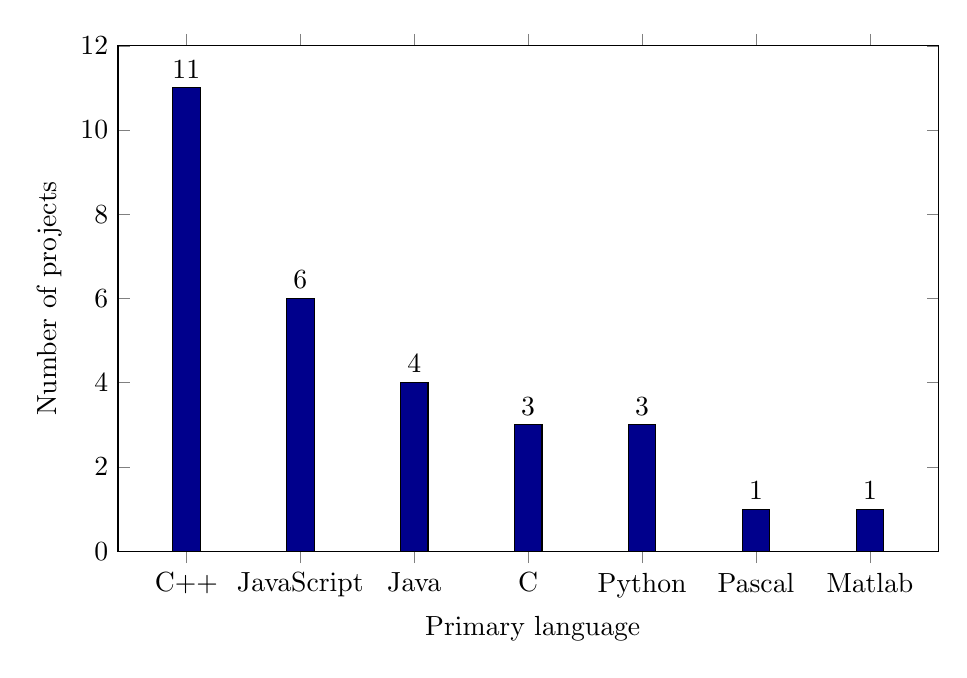
\begin{tikzpicture}
\centering
\begin{axis}
[
ybar,
height=8cm,
width=12cm,
ylabel={Number of projects},
xlabel={\ Primary language},
symbolic x coords={C++, JavaScript, Java, C, Python, Pascal, Matlab},
xtick=data,
nodes near coords,
nodes near coords align={vertical},
]
\addplot[black,fill=blue!55!black] coordinates {(C++,11) (JavaScript,6) (Java,4) (C,3) (Python,3) (Pascal,1) (Matlab,1) };
\end{axis}  
\end{tikzpicture}
\caption{\label{fig_language}Primary languages versus number of projects using them}
\end{figure}

We failed to install \textit{DICOM Viewer}, so we could not test its \textit{surface reliability} and \textit{surface robustness}. We kept this software on our list because the other seven qualities do not rely on a successful installation. Besides, the \textit{DICOM Viewer} team built it as a plugin software for NextCloud (\hyperlink{https://apps.nextcloud.com/}{https://apps.nextcloud.com/}) platform, which was a unique choice we had not seen before. We wanted to keep it to enrich the diversity.

\section{Installability}
\label{sec_result_installability}

Figure \ref{fg_installability_scores} lists the scores of \textit{installability}.

\begin{figure}[H]
\includegraphics[scale=0.38]{figures/installability_scores.png}
\caption{AHP installability scores}
\label{fg_installability_scores}
\end{figure}

We found installation instructions for 16 projects. Among the ones without instructions, \textit{BioImage Suite Web} and \textit{Slice:Drop} are web applications with online versions to use, thus they do not need installation. Installing 10 of the projects required extra dependencies. Five of them are the web applications in Table \ref{tab_final_list}, and depended on a browser; \textit{dwv}, \textit{OHIF Viewer}, and \textit{GATE} needed extra dependencies to build; \textit{ImageJ} and	\textit{Fiji} needed an unzip tool; \textit{MatrixUser} was based on Matlab; \textit{DICOM Viewer} needed to work on a Nextcloud platform.

\textit{3D Slicer} has the highest score because it had easy to follow installation instructions, and the installation processes were automated, fast, and frustration-free, with all dependencies automatically added. There were also no errors during the installation and uninstallation steps. Many other software packages also had installation instructions and automated installers, and we had no trouble installing them, such as \textit{INVESALIUS 3}, \textit{Gwyddion}, \textit{XMedCon}, and \textit{MicroView}. We gave them various scores based on the understandability of the instructions, installation steps, and user experience. Since \textit{BioImage Suite Web} and \textit{Slice:Drop} needed no installation, we gave them higher scores. \textit{BioImage Suite Web} also provided an option to download cache to local for offline usage, which was easy to apply.

\textit{dwv}, \textit{GATE}, and \textit{DICOM Viewer} showed severe problems. We could not install them. We spent a reasonable amount of time on these problems, then considered them as major obstacles for normal users if we could not figure out any solutions. We suspect that only a part of the users faced the same problems, and given a lot of time, we might be able to find solutions. However, the difficulties greatly impacted the installation experiences, and we graded these software packages with lower scores. For example, \textit{dwv} and \textit{GATE} had the option to build from the source code, and we failed the building processes following the instructions. Although we could not locally build them, we could use a deployed online version for \textit{dwv}, and a VM version for \textit{GATE}. With those, we finished all the measurements for them. Furthermore, \textit{DICOM Viewer} depended on the NextCloud platform, and we could not successfully install the dependency.

\textit{MatrixUser} has a lower score because it depended on Matlab. We considered installing Matlab takes many more steps and time, and some users may not have a license to use Matlab.

\section{Correctness \& Verifiability}
\label{sec_result_correctness_verifiability}

The scores of \textit{correctness \& verifiability} are shown in Figure \ref{fg_correctness_erifiability_scores}. Generally speaking, the packages with higher scores adopted more techniques to improve \textit{correctness}, and had better documents for us to verify it.

\begin{figure}[H]
\includegraphics[scale=0.38]{figures/correctness_verifiability_scores.png}
\caption{AHP correctness \& verifiability scores}
\label{fg_correctness_erifiability_scores}
\end{figure}

After examining the source code, we could not find any evidence of unit testing in more than half of the projects. Unit testing benefits most parts of the software's life cycle, such as designing, coding, debugging, and optimization \cite{Hamill2004}. It can reveal the bugs at an earlier stage of the development process, and the absence of unit testing may cause problems for \textit{correctness \& verifiability}.

We could not find requirements specifications for most projects. The only document we found is a road map of \textit{3D Slicer}, which contained design requirements for the upcoming changes. However, it did not record the conditions for previous versions. We also could not identify the theory manuals for all of the projects. Even for some projects with well-organized documents, requirements specifications and theory manuals were still missing.

We identified five projects using CI/CD tools, which are \textit{3D Slicer}, \textit{ImageJ
}, \textit{Fiji}, \textit{dwv}, and \textit{OHIF Viewer}.

In this section, the information about CI/CD tools is part of the answers to \hyperlink{rq2}{RQ2}, and the information about software testing and documentation is part of the answers to \hyperlink{rq3}{RQ3}.

\section{Surface Reliability}
\label{sec_result_reliability}
As described in Section \ref{sec_result_installability}, we could not build \textit{dwv} and \textit{GATE}. However, since there was an online or VM version of them, successful deployment is possible. So the failure of installation did not affect their scores in \textit{surface reliability}. Figure \ref{fg_reliability_scores} shows the AHP results.

\begin{figure}[H]
\includegraphics[scale=0.38]{figures/reliability_scores.png}
\caption{AHP surface reliability scores}
\label{fg_reliability_scores}
\end{figure}

As shown in Section \ref{sec_result_installability}, most of the software products did not ``break" during installation or did not need installation; \textit{dwv} and \textit{GATE} broke in the building stage, and the processes were not recoverable; we could not install the dependency for \textit{DICOM Viewer}.

Of the seven software packages with a getting started tutorial and operation steps in the tutorial, most showed no error when we followed the steps. However, \textit{GATE} could not open macro files and became unresponsive several times, without any descriptive error message. When assessing \textit{surface robustness} (Section \ref{sec_result_robustness}), we found out that \textit{Drishti} crashed during loading damaged image files and did not show any descriptive error message. On the other hand, we did not see any problems with the online version of \textit{dwv}.

\section{Surface Robustness}
\label{sec_result_robustness}
Figure \ref{fg_robustness_scores} presents the scores for \textit{surface robustness}.

\begin{figure}[H]
\includegraphics[scale=0.38]{figures/robustness_scores.png}
\caption{AHP surface robustness scores}
\label{fg_robustness_scores}
\end{figure}

The packages with higher scores elegantly handled the unexpected/unanticipated inputs, typically showing a clear error message. We might underestimate the score of \textit{OHIF Viewer} since we needed further customization to load data, and the test was not complete.

Digital Imaging and Communications in Medicine (DICOM) is a widely used MI standard, and ``it defines the formats for medical images that can be exchanged with the data and quality necessary for clinical use" \cite{MITA2021}. According to their documentation, all 29 software packages should support the DICOM standard. We prepared two types of image files: the ones in correct formats and the broken ones. We used two MI sample files in the DICOM format as the image files with valid formats; we created a standard text file, changed its extension name from ``.txt" to ``.dcm", and used it as the unexpected/unanticipated input.

Being tested with the input files with correct formats, all software packages except \textit{GATE} loaded the images correctly. \textit{GATE} failed this test for unknown reasons.

With the unexpected/unanticipated input, \textit{MatrixUser}, \textit{dwv}, and \textit{Slice:Drop} ignored the incorrect format of the file and loaded it regardless. They did not show any error message and displayed a blank image. \textit{MRIcroGL} behaved similarly except that it showed a meaningless image with noise pixels. \textit{Drishti} successfully detected the broken format of the file, but the software crashed as a result. We recorded \textit{Drishti}'s issue to the measurement of its \textit{reliability} in Section \ref{sec_result_installability}.

\section{Surface Usability}
\label{sec_result_usability}
Figure \ref{fg_usability_scores} lists the AHP scores for \textit{surface usability}.

\begin{figure}[H]
\includegraphics[scale=0.38]{figures/usability_scores.png}
\caption{AHP surface usability scores}
\label{fg_usability_scores}
\end{figure}

We found a getting started tutorial for only 11 projects but a user manual for 22 projects. \textit{MRIcroGL} was the only one with documentation for the expected user characteristics.

The software with higher scores usually provided both comprehensive document guidance and a good user experience. \textit{INVESALIUS 3} set an excellent example of a detailed and precise user manual. \textit{GATE} also provided a large number of documents, but we think that they conveyed the ideas poorly, as we had trouble understanding and using them.
 
Table \ref{tab_user_support_model} shows the user support models by the number of projects using them. This table contains part of the answers to \hyperlink{rq2}{RQ2}. Maybe not every team intended to use GitHub issues to answer users' questions, but many users use them to seek help.

\begin{table}[H]
\centering
\begin{tabular}{ll}
\hline
\multicolumn{1}{c}{User support model} & Number of projects \\ \hline
GitHub issue & 24 \\
Frequently Asked Questions (FAQ) & 12 \\
Forum & 10 \\
E-mail address & 9 \\
GitLab issue, SourceForge discussions & 2 \\
Troubleshooting & 2 \\
Contact form & 1 \\ \hline
\end{tabular}
\caption{\label{tab_user_support_model}User support models by number of projects}
\end{table}

\section{Maintainability}
\label{sec_score_maintainability}
Figure \ref{fg_maintainability_scores} shows the AHP results for \textit{maintainability}. 

\begin{figure}[H]
\includegraphics[scale=0.38]{figures/maintainability_scores.png}
\caption{AHP maintainability scores}
\label{fg_maintainability_scores}
\end{figure}

We marked \textit{3D Slicer} with a much higher score than others because it did very well at closing the identified issues, and more importantly, we found it to have the most comprehensive artifacts. For example, as far as we could find out, only a few of the 29 projects had a project plan, developer's manual, or API documentation, and only \textit{3D Slicer}, \textit{ImageJ}, \textit{Fiji} included all three documents. Meanwhile, \textit{3D Slicer} has a much higher percentage of closed issues (91.65\%) than \textit{ImageJ} (52.49\%) and \textit{Fiji} (63.79\%). Table \ref{tab_maintainability_docs} shows which projects had these documents, in the descending order of their \textit{maintainability} scores. This table contains part of the answers to \hyperlink{rq1}{RQ1} and \hyperlink{rq3}{RQ3}.

\begin{table}[H]
\centering
\begin{tabular}{llll}
\hline
\multicolumn{1}{c}{Software} & Proj plan & Dev manual & API doc \\ \hline
3D Slicer & X & X & X \\
ImageJ & X & X & X \\
Weasis &  & X &  \\
OHIF Viewer &  & X & X \\
Fiji & X & X & X \\
ParaView & X &  &  \\
SMILI &  &  & X \\
medInria &  & X &  \\
INVESALIUS 3 & X &  &  \\
dwv &  &  & X \\
BioImage Suite Web &  & X &  \\
Gwyddion &  & X & X \\ \hline
\end{tabular}
\caption{\label{tab_maintainability_docs}Software with the maintainability documents}
\end{table}

27 of the 29 projects used git as the version control tool; \textit{AMIDE} used Mercurial; \textit{Gwyddion} used Subversion. 24 projects used GitHub for their repositories; \textit{XMedCon
}, \textit{AMIDE}, and \textit{Gwyddion} used SourceForge; \textit{DicomBrowser} and \textit{3DimViewer} used BitBucket. The information about version control tools is part of the answers to \hyperlink{rq2}{RQ2}.

\section{Reusability}
\label{sec_result_reusability}
Figure 4.7 shows the AHP results for \textit{reusability}.

\begin{figure}[H]
\includegraphics[scale=0.38]{figures/reusability_scores.png}
\caption{AHP reusability scores}
\label{fg_reusability_scores}
\end{figure}

As described in Section \ref{sec_grading_template}, we gave higher scores to the projects with an API document. As shown in Table \ref{tab_maintainability_docs}, seven projects had API documents. We also considered projects with more code files and less LOC per code file as more reusable. Table \ref{tab_loc_per_file} shows the number of text-based files by projects, which we used to approximate the number of code files. The table also lists the total number of lines (including comments and blanks), LOC, and average LOC per file. We arranged the items in the descending order of their \textit{reusability} scores. 

\begin{table}[H]
\centering
\begin{tabular}{lllll}
\hline
\multirow{2}{*}{Software} & \multirow{2}{*}{Text files} & \multirow{2}{*}{Total lines} & \multirow{2}{*}{LOC} & \multirow{2}{*}{LOC/file} \\
 &  &  &  &  \\ \hline
OHIF Viewer & 1162 & 86306 & 63951 & 55 \\
3D Slicer & 3386 & 709143 & 501451 & 148 \\
Gwyddion & 2060 & 787966 & 643427 & 312 \\
ParaView & 5556 & 1276863 & 886326 & 160 \\
OsiriX Lite & 2270 & 873025 & 544304 & 240 \\
Horos & 2346 & 912496 & 561617 & 239 \\
medInria & 1678 & 214607 & 148924 & 89 \\
Weasis & 1027 & 156551 & 123272 & 120 \\
BioImage Suite Web & 931 & 203810 & 139699 & 150 \\
GATE & 1720 & 311703 & 207122 & 120 \\
Ginkgo CADx & 974 & 361207 & 257144 & 264 \\
SMILI & 275 & 90146 & 62626 & 228 \\
Fiji & 136 & 13764 & 10833 & 80 \\
Drishti & 757 & 345225 & 268168 & 354 \\
ITK-SNAP & 677 & 139880 & 88530 & 131 \\
3DimViewer & 730 & 240627 & 178065 & 244 \\
DICOM Viewer & 302 & 34701 & 30761 & 102 \\
ImageJ & 40 & 10740 & 9681 & 242 \\
dwv & 188 & 71099 & 47815 & 254 \\
MatrixUser & 216 & 31336 & 23121 & 107 \\
INVESALIUS 3 & 156 & 59328 & 48605 & 312 \\
AMIDE & 183 & 139658 & 102827 & 562 \\
Papaya & 110 & 95594 & 71831 & 653 \\
MicroView & 137 & 36173 & 27470 & 201 \\
XMedCon & 202 & 129991 & 96767 & 479 \\
MRIcroGL & 97 & 50445 & 8493 & 88 \\
Slice:Drop & 77 & 25720 & 19020 & 247 \\
DicomBrowser & 54 & 7375 & 5505 & 102 \\
dicompyler & 48 & 19201 & 15941 & 332 \\ \hline
\end{tabular}
\caption{\label{tab_loc_per_file}Number of files and lines}
\end{table}

\section{Surface Understandability}
\label{sec_result_understandability}
Figure \ref{fg_surface_understandability_scores} shows the scores for \textit{surface understandability}.

\begin{figure}[H]
\includegraphics[scale=0.38]{figures/understandability_scores.png}
\caption{AHP surface understandability scores}
\label{fg_surface_understandability_scores}
\end{figure}

All projects had a consistent code style with parameters in the same order for all functions; the code was modularized; the comments were clear, indicating what is being done, not how. However, we only found explicit identification of a coding standard for 3 out of the 29: \textit{3D Slicer}, \textit{Weasis}, and \textit{ImageJ}. We also found hard-coded constants in \textit{medInria}, \textit{dicompyler}, \textit{MicroView}, and \textit{Papaya}. We did not find any reference to the used algorithms in projects \textit{XMedCon}, \textit{DicomBrowser}, \textit{3DimViewer}, \textit{BioImage Suite Web}, \textit{Slice:Drop}, \textit{MatrixUser}, \textit{DICOM Viewer}, \textit{dicompyler}, and \textit{Papaya}. 

\section{Visibility/Transparency}
\label{sec_result_visibility_transparency}
Figure \ref{fg_visibility_transparency_scores} shows the AHP scores for \textit{visibility/transparency}. Generally speaking, the teams that actively documented their development process and plans scored higher because they delivered better communication to people outside the team.

\begin{figure}[H]
\includegraphics[scale=0.38]{figures/visibility_transparency_scores.png}
\caption{AHP visibility/transparency scores}
\label{fg_visibility_transparency_scores}
\end{figure}

Table \ref{tab_Visibility/Transparency_docs} shows the projects which had documents for the development process, project status, development environment, and release notes, in the descending order of their \textit{visibility/transparency} scores. This table contains part of the answers to \hyperlink{rq1}{RQ1} and \hyperlink{rq3}{RQ3}.

\begin{table}[H]
\centering
\begin{tabular}{lllll}
\hline
Software & Dev process & Proj status & Dev env & Rls notes \\ \hline
3D Slicer & X & X & X & X \\
ImageJ & X & X & X & X \\
Fiji & X & X & X &  \\
MRIcroGL &  &  &  & X \\
Weasis &  &  & X & X \\
ParaView &  & X &  &  \\
OHIF Viewer &  &  & X & X \\
DICOM Viewer &  &  & X & X \\
medInria &  &  & X & X \\
SMILI &  &  &  & X \\
Drishti &  &  &  & X \\
INVESALIUS 3 &  &  &  & X \\
OsiriX Lite &  &  &  & X \\
GATE &  &  &  & X \\
MicroView &  &  &  & X \\
MatrixUser &  &  &  & X \\
BioImage Suite Web &  &  & X &  \\
ITK-SNAP &  &  &  & X \\
Horos &  &  &  & X \\
dwv &  &  &  & X \\
Gwyddion &  &  &  & X \\ \hline
\end{tabular}
\caption{\label{tab_Visibility/Transparency_docs}Software with the visibility/transparency documents}
\end{table}

\section{Overall Scores}

As described in Section \ref{sec_AHP}, for our AHP measurements, there are nine criteria which are the nine software qualities and 29 software packages as the alternatives. In the absence of requirements for an actual project, we made all nine qualities equally important, so the score of each quality affects the overall scores on the same scale.

Figure \ref{fg_overall_scores} shows the overall scores of all 29 software packages in descending order. Since we produced the scores from the AHP process, the total sum of the 29 scores is precisely 1.

\begin{figure}[H]
\includegraphics[scale=0.38]{figures/overall_scores.png}
\caption{Overall AHP scores for all 9 software qualities}

\label{fg_overall_scores}
\end{figure}

The top three software products \textit{3D Slicer}, \textit{ImageJ}, and \textit{OHIF Viewer} had higher scores in most criteria. \textit{3D Slicer} ranked in the top two software products for all qualities except \textit{surface robustness}; \textit{ImageJ} ranked in the top three products for \textit{correctness \& verifiability}, \textit{surface reliability}, \textit{surface usability}, \textit{maintainability}, \textit{ surface understandability}, and \textit{visibility/transparency}; \textit{OHIF Viewer} ranked in the top five products for \textit{correctness \& verifiability}, \textit{surface reliability}, \textit{surface usability}, \textit{maintainability}, and \textit{reusability}. We might underestimate its scores of qualities \textit{surface reliability} and \textit{surface robustness} for \textit{DICOM Viewer}, but equally compared it with the other software for the rest seven qualities.

\chapter{Interviews with Developers}
\label{ch_interviews}

\section{Summary of Answers}

\begin{itemize}
\item Start with one by one, with commonalities and interesting special cases.

\item Shorten and summarize later.
\end{itemize}

\section{Discussions}

Any conclusions?

\chapter{Recommendations}
\label{ch_recommendations}

I think the recommendations can originate from both parts - measurements and interviews.
\include{17Conclusion}

\addcontentsline{toc}{chapter}{Bibliography}
%\bibliographystyle{plain}
\bibliography{thesis}


\appendix
\chapter{Full Grading Template}
\label{ap_grading_template}

\newpage
\begingroup
\renewcommand{\arraystretch}{0.8}

\begin{table}[H]
\centering
\caption{Measurement Template}\label{measurementtemplate}
\begin{tabular}{p{14cm}}
\hline
\textbf{Summary Information}\\
\hline
Software name? (string)\\
URL? (URL)\\
Affiliation (institution(s)) (string or {N/A})\\
Software purpose (string)\\
Number of developers (all developers that have contributed at least one commit to the project) (use repo commit logs) (number)\\
How is the project funded? (unfunded, unclear, funded$\ast$) where $\ast$ requires a string to say the source of funding\\
Initial release date? (date)\\
Last commit date? (date)\\
Status? (alive is defined as presence of commits in the last 18 months) ({alive, dead, unclear})\\
License? ({GNU GPL, BSD, MIT, terms of use, trial, none, unclear, other$\ast$}) $\ast$ given via a string \\
Platforms? (set of {Windows, Linux, OS X, Android, other$\ast$}) $\ast$ given via string\\
Software Category? The concept category includes software that does not have an officially released version. Public software has a released version in the public domain. Private software has a released version available to authorized users only. ({concept, public, private})\\
Development model? ({open source, freeware, commercial, unclear})\\
Publications about the software? Refers to publications that have used or mentioned the software. (number or {unknown})\\
Source code URL? ({set of url, n/a, unclear})\\
Programming language(s)? (set of {FORTRAN, Matlab, C, C++, Java, R, Ruby, Python, Cython, BASIC, Pascal, IDL, unclear, other$\ast$}) $\ast$ given via string \\
Is there evidence that performance was considered? Performance refers to either speed, storage, or throughput. ({yes$\ast$, no})\\
Additional comments? (can cover any metrics you feel are missing, or any other thoughts you have) \\
\hline
\end{tabular}
\end{table}

\begin{table}[H]
\centering
\begin{tabular}{p{14cm}}
\hline		
\textbf{Installability  (Measured via installation on a virtual machine.) }\\
\hline
Are there installation instructions? ({yes, no})\\
Are the installation instructions in one place? Place referring to a single document or web-page. ({yes, no, n/a})\\
Are the installation instructions linear? Linear meaning progressing  in a single series of steps. ({yes, no, n/a})\\
Are the instructions written as if the person doing the installation has none of the dependent packages installed? ({yes, no, unclear})\\
Are compatible operating system versions listed? ({yes, no})\\
Is there something in place to automate the installation (makefile, script, installer, etc)? ({yes$\ast$, no})\\
If the software installation broke, was a descriptive error message displayed? ({yes, no, n/a})\\
Is there a specified way to validate the installation? ({yes$\ast$, no})\\
How many steps were involved in the installation? (Includes manual steps like unzipping files) Specify OS. (number, OS)\\
What OS was used for the installation? ({Windows, Linux, OS X, Android, other$\ast$ }) $\ast$given via string\\
How many extra software packages need to be installed before or during installation? (number)\\
Are required package versions listed? ({yes, no, n/a})\\
Are there instructions for the installation of required packages / dependencies? ({yes, no, n/a})\\
Run uninstall, if available. Were any obvious problems caused? ({yes$\ast$ , no, unavail})\\
Overall impression? ({1 .. 10})\\
Additional comments? (can cover any metrics you feel are missing, or any other thoughts you have)\\
\hline
\end{tabular}
\end{table}

\begin{table}[H]
\centering
\begin{tabular}{p{14cm}}
\hline		
\textbf{Correctness and Verifiability}\\
\hline
Any reference to the requirements specifications of the program or theory manuals? ({yes$\ast$ , no, unclear})\\
What tools or techniques are used to build confidence of correctness? ({literate programming, automated testing, symbolic execution, model checking, assertions used in the code, Sphinx, Doxygen, Javadoc, confluence, unclear, other$\ast$}) $\ast$ given via string\\
If there is a getting started tutorial? ({yes, no})\\
Are the tutorial instructions linear? ({yes, no, n/a})\\
Does the getting started tutorial provide an expected output? ({yes, no$\ast$, n/a})\\
Does your tutorial output match the expected output? ({yes, no, n/a})\\
Are unit tests available?  ({yes, no, unclear})\\
Is there evidence of continuous integration? (for example mentioned in documentation, Jenkins, Travis CI, Bamboo, other) ({yes$\ast$, no, unclear})\\
Overall impression? ({1 .. 10})\\
Additional comments? (can cover any metrics you feel are missing, or any other thoughts you have) \\
\hline	
\textbf{Surface Reliability}\\
\hline
Did the software “break” during installation? ({yes$\ast$ , no})\\
If the software installation broke, was the installation instance recoverable? ({yes, no, n/a})\\
Did the software “break” during the initial tutorial testing? ({yes$\ast$, no, n/a})\\
If the tutorial testing broke, was a descriptive error message displayed? ({yes, no, n/a})\\
If the tutorial testing broke, was the tutorial testing instance recoverable? ({yes, no, n/a})\\
Overall impression? ({1 .. 10})\\
Additional comments? (can cover any metrics you feel are missing, or any other thoughts you have)\\
\hline		
\end{tabular}
\end{table}

\begin{table}[H]
\centering
\begin{tabular}{p{14cm}}
\hline		
\textbf{Surface Robustness}\\
\hline
Does the software handle unexpected/unanticipated input (like data of the wrong type, empty input, missing files or links) reasonably? (a reasonable response can include an appropriate error message.) ({yes, no$\ast$ })\\
For any plain text input files, if all new lines are replaced with new lines and carriage returns, will the software handle this gracefully? ({yes, no$\ast$, n/a})\\
Overall impression? ({1 .. 10})\\
Additional comments? (can cover any metrics you feel are missing, or any other thoughts you have)\\
\hline		
\textbf{Surface Usability}\\
\hline
Is there a getting started tutorial? ({yes, no})\\
Is there a user manual? ({yes, no})\\
Are expected user characteristics documented? ({yes, no})\\
What is the user support model? FAQ? User forum? E-mail address to direct questions? Etc. (string)\\
Overall impression? ({1 .. 10})\\
Additional comments? (can cover any metrics you feel are missing, or any other thoughts you have)\\
\hline
\end{tabular}
\end{table}

\begin{table}[H]
\begin{tabular}{p{14cm}}
\hline	
\textbf{Maintainability}\\
\hline
What is the current version number? (number)\\
Is there any information on how code is reviewed, or how to contribute? ({yes$\ast$, no})\\
Are artifacts available? (List every type of file that is not a code file – for examples please look at the ‘Artifact Name’ column of https://gitlab.cas.mcmaster.ca/SEforSC/se4sc/-/blob/git-svn/GradStudents/Olu/ResearchProposal/Artifacts\_MiningV3.xlsx) ({yes$\ast$, no, unclear}) $\ast$list via string\\
What issue tracking tool is employed? (set of {Trac, JIRA, Redmine, e-mail, discussion board, sourceforge, google code, git, BitBucket, none, unclear, other$\ast$}) $\ast$ given via string\\
What is the percentage of identified issues that are closed? (percentage)\\
What percentage of code is comments? (percentage)\\
Which version control system is in use? ({svn, cvs, git, github, unclear, other$\ast$}) $\ast$ given via string\\
Overall impression? ({1 .. 10})\\
Additional comments? (can cover any metrics you feel are missing, or any other thoughts you have)\\
\hline		
\textbf{Reusability}\\
\hline
How many code files are there? (number)\\
Is API documented? ({yes, no, n/a})\\
Overall impression? ({1 .. 10})\\
Additional comments? (can cover any metrics you feel are missing, or any other thoughts you have)\\
\hline		
\end{tabular}
\end{table}

\begin{table}[H]
\begin{tabular}{p{14cm}}
\hline		
\textbf{Surface Understandability (Based on 10 random source files)}\\
\hline
Consistent indentation and formatting style? ({yes, no, n/a})\\
Explicit identification of a coding standard? ({yes$\ast$, no, n/a})\\
Are the code identifiers consistent, distinctive, and meaningful? ({yes, no$\ast$ , n/a})\\
Are constants (other than 0 and 1) hard coded into the program? ({yes, no$\ast$ , n/a})\\
Comments are clear, indicate what is being done, not how? ({yes, no$\ast$ , n/a})\\
Is the name/URL of any algorithms used mentioned? ({yes, no$\ast$ , n/a})\\
Parameters are in the same order for all functions? ({yes, no$\ast$ , n/a})\\
Is code modularized? ({yes, no$\ast$ , n/a})\\
Overall impression? ({1 .. 10})\\
Additional comments? (can cover any metrics you feel are missing, or any other thoughts you have)\\
\hline		
\textbf{Visibility/Transparency}\\
\hline
Is the development process defined? If yes, what process is used. ({yes$\ast$, no, n/a})\\
Are there any documents recording the development process and status?  ({yes$\ast$, no}))\\
Is the development environment documented? ({yes$\ast$, no})\\
Are there release notes? ({yes$\ast$, no})\\
Overall impression? ({1 .. 10})\\
Additional comments? (can cover any metrics you feel are missing, or any other thoughts you have)\\
\hline
\end{tabular}
\end{table}

\begin{table}[H]
\begin{tabular}{p{14cm}}
\hline		
\textbf{Raw Metrics (Measured via git\_stats)}\\
\hline
Number of text-based files. (number)\\
Number of binary files. (number)\\
Number of total lines in text-based files. (number)\\
Number of total lines added to text-based files. (number)\\
Number of total lines deleted from text-based files. (number)\\
Number of total commits. (number)\\
Numbers of commits by year in the last 5 years. (Count from as early as possible if the project is younger than 5 years.) (list of numbers)\\
Numbers of commits by month in the last 12 months. (list of numbers)\\
\hline		
\textbf{Raw Metrics (Measured via scc)}\\
\hline
Number of text-based files. (number)\\
Number of total lines in text-based files. (number)\\
Number of code lines in text-based files. (number)\\
Number of comment lines in text-based files. (number)\\
Number of blank lines in text-based files. (number)\\
\hline
\textbf{Repo Metrics (Measured via GitHub)}\\
\hline
Number of people watching this repo. (number)\\
Number of stars. (number)\\
Number of forks. (number)\\
Number of open pull requests. (number)\\
Number of closed pull requests. (number)\\
Number of months on GitHub. (number)\\
Accessed date. (date)\\
\hline
\end{tabular}
\end{table}

\endgroup
\chapter{Summary of Measurements}
\label{ap_measurements}

appendix here
\chapter{Other Interview Answers}
\label{ap_interview}

We asked 20 interview questions to the nine interviewees from eight software projects. We discuss the answers to interview questions 5, 9, 10, 11, 12, 13, 14, and 19 in Section \ref{ch_interview}, and summarize the answers to the other questions in this section.

\noindent\textbf{Q1. Interviewees’ current position/title? degrees?}

Six of the nine interviewees revealed their position/title, such as CEO of a company, endowed chair and professor in universities, software engineers in a commercial company and a hospital.

Most of them answered their backgrounds and degrees. Table \ref{tab_q1_degrees} shows the highest academic degrees the participants have, and Table \ref{tab_q1_majors} shows what majors they studied. Many of the interviewees studied in multiple majors.

\begin{table}[H]
\centering
\begin{tabular}{ll}
\hline
Highest degree & Number of interviewees \\ \hline
PHD & 4 \\
Master & 3 \\
Bachelor & 0 \\
Unspecified academic degree & 2 \\ \hline
\end{tabular}
\caption{\label{tab_q1_degrees}Interviewees' highest academic degrees}
\end{table}

\begin{table}[H]
\centering
\begin{tabular}{ll}
\hline
Major & Number of interviewees \\ \hline
Computer Science & 4 \\
Physics & 2 \\
Biomedical Engineering & 1 \\
Neuroimaging & 1 \\
Geology (image analysis) & 1 \\
Media Arts and Sciences & 1 \\
Mechanical Engineering & 1 \\
Materials Engineering & 1 \\
Psychology & 1 \\ \hline
\end{tabular}
\caption{\label{tab_q1_majors}Interviewees' majors at university}
\end{table}

\noindent\textbf{Q2. Interviewees’ contribution to/relationship with the software?}

Table \ref{tab_q2_roles} shows the interviewees’ roles and responsibilities in the projects. One of the participants did not explicitly mention his role, but implicitly revealed that he was a primary contributor to the project.

\begin{table}[H]
\centering
\begin{tabular}{ll}
\hline
Role in the projects & Number of interviewees \\ \hline
Chief Architect & 2 \\
Lead Developer & 1 \\
Core Developer & 5 \\
Unspecified & 1 \\ \hline
\end{tabular}
\caption{\label{tab_q2_roles}Interviewees' roles in the projects}
\end{table}

\noindent\textbf{Q3. Length of time the interviewee has been involved with this software?}

Table \ref{tab_q3_years} shows the distribution of the lengths of time the interviewees had worked on the projects.

\begin{table}[H]
\centering
\begin{tabular}{ll}
\hline
Length of time in the projects & Number of interviewees \\ \hline
0-1 & 1 \\
2-5 & 0 \\
6-10 & 2 \\
11-15 & 3 \\
16-20 & 2 \\
21-25 & 1 \\ \hline
\end{tabular}
\caption{\label{tab_q3_years}Lengths of time that the interviewees worked in the projects}
\end{table}

\noindent\textbf{Q4. How large is the development group?}

The size of each group grows and shrinks over the years. Most teams mentioned that the team members join and leave. Some teams said that when there was sufficient funding, they could afford more developers.

Table \ref{tab_q4_members} shows the numbers of active members at the time of interviews. The members include people working on development and project management.

\begin{table}[H]
\centering
\begin{tabular}{ll}
\hline
Number of current members & Number of projects \\ \hline
1-3 & 5 \\
4-6 & 3 \\ \hline
\end{tabular}
\caption{\label{tab_q4_members}Numbers of current members in the projects}
\end{table}

As shown in the table, no team had a vast number of members. Some projects had more developers, such as \textit{3D Slicer}; on the other hand, some teams such as \textit{dwv} had only one primary developer, plus a maximum of two or three developers occasionally.

\textit{3D Slicer} is a special case, because it supports third-party extensions. So there have been community members developing and maintaining these extensions. Table \ref{tab_q4_members} does not include these members.

\noindent\textbf{Q6. What is the typical background of a developer?}

Not all interviewees could clearly answer this question. Many of them talked about the backgrounds of members with who they were familiar. Table \ref{tab_q6_dev_backgrounds} shows the number of times all interviewees mentioned a background.

\begin{table}[H]
\centering
\begin{tabular}{ll}
\hline
Background of a developer & Number of interviewees with the answer \\ \hline
\begin{tabular}[c]{@{}l@{}}Computer Science, Information\\ Technology, and Software Development \end{tabular} & 6 \\
Imaging & 2 \\
Medical Imaging & 1 \\
Mathematics & 1 \\
Biomedical Engineering & 1 \\
Computer Aided Medical Procedures & 1 \\
Physician & 1 \\ \hline
\end{tabular}
\caption{\label{tab_q6_dev_backgrounds}Backgrounds of developers by the numbers of interviewees with the answers}
\end{table}

\noindent\textbf{Q7. What is your estimated number of users? How did you come up with that estimate?}

None of the interviewees knew the exact number of users. Some of them provided estimations based on different facts. However, we do not think these numbers are comparable to each other.

\begin{table}[H]
\centering
\begin{tabular}{lll}
\hline
Software & Rough estimation & Considered facts \\ \hline
3D Slicer & 100,000 & \begin{tabular}[c]{@{}l@{}} Search results on Google Scholar;\\ number of new posts per year on slicer.org; \\ number of downloads. \end{tabular} \\
INVESALIUS 3 & 75,000 & Number of random IDs created by new installation.\\
dwv & No estimation & About 20 companies integrated \textit{dwv} in their products. \\
BioImage Suite Web & 100 active users & \begin{tabular}[c]{@{}l@{}}  The  interviewee only counted the users from \\ several Universities who were active users. \end{tabular} \\
ITK-SNAP & 10,000 plus & Number of downloads. \\
MRIcroGL & No estimation & \begin{tabular}[c]{@{}l@{}}  It is the top 1 downloaded software on this NITRC list \\ \hyperlink{https://www.nitrc.org/top/toplist.php?type=downloads}{https://www.nitrc.org/top/toplist.php?type=downloads} \end{tabular} \\
Weasis & \begin{tabular}[c]{@{}l@{}}  10,000 user used \\ it as least once \end{tabular} & Number of profiles. \\
OHIF & About 5000 & \begin{tabular}[c]{@{}l@{}}   Some platforms integrated \textit{OHIF}, and it was hard \\ to know the number of end users. \end{tabular} \\ \hline
\end{tabular}
\caption{\label{tab_q7_num_users}Rough Estimations for the Number of Users}
\end{table}

Table \ref{tab_q7_num_users} shows the estimations and how the interviewees made them. It is clear that some estimated only the active users, and some counted users who had used only once. So we do not compare these numbers.

\noindent\textbf{Q8. What is the typical background of a user?}

All interviewees provided several different user backgrounds, and all of them mentioned medical researchers or medical professionals. Table \ref{tab_q8_user_backgrounds} shows the number of times all interviewees mentioned a background.

\begin{table}[H]
\centering
\begin{tabular}{ll}
\hline
Background of a user & Number of interviewees with the answer \\ \hline
Medical Researchers & 6 \\
Doctors/Health care professionals/Surgeons & 5 \\
Student Researchers & 4 \\
Patients & 3 \\
Paleontologist & 1 \\
Biomechanical Engineers & 1 \\
Imaging Researchers & 1 \\
Mechanical Engineers & 1 \\ \hline
\end{tabular}
\caption{\label{tab_q8_user_backgrounds}Backgrounds of users by the numbers of interviewees with the answers}
\end{table}


\end{document}
